\clearpage
\begin{proofbox}
\textbf{统一约定：}$a,b>0$，$P(x,y)\in H$，
两渐近线 $\ell_\pm:bx\mp ay=0$。$OQPR$ 如陈述中所定义，$S>0$。
以下提供\textbf{最快法、最低门槛法、常规法}，再补充向量的通用做法。

\medskip
\textbf{方法一：最快证明【两组平行线间距＋夹角；3 步】。}

\begin{center}
% a=3,b=2; u=9/4,v=1. Orthogonal feet are computed exactly.
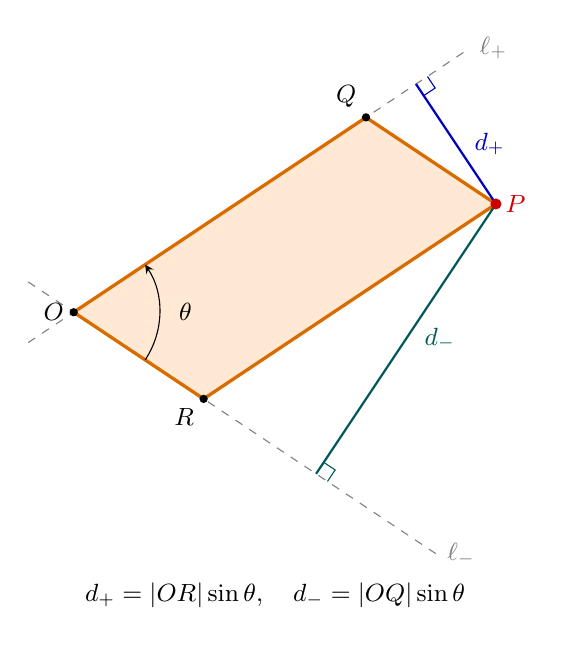
\begin{tikzpicture}[x=1.65cm,y=1.65cm,>=stealth,font=\small]
\coordinate (O) at (0,0); \coordinate (Q) at (2.25,1.5);
\coordinate (R) at (1,-2/3); \coordinate (P) at (3.25,5/6);
\coordinate (A) at (137/52,137/78);
\coordinate (B) at (97/52,-97/78);
\fill[orange!17] (O)--(Q)--(P)--(R)--cycle;
\draw[gray,dashed] (-.35,-7/30)--(3.05,61/30) node[right] {$\ell_+$};
\draw[gray,dashed] (-.35,7/30)--(2.8,-28/15) node[right] {$\ell_-$};
\draw[orange!85!black,very thick] (O)--(Q)--(P)--(R)--cycle;
\draw[blue!75!black,thick] (P)--(A) node[midway,right=3pt] {$d_+$};
\draw[teal!70!black,thick] (P)--(B) node[midway,right=3pt] {$d_-$};
% right angle markers at A and B
\draw[blue!75!black] (2.7231,1.8141)--(2.7819,1.7259)--(2.6937,1.6671);
\draw[teal!70!black] (1.9536,-1.3024)--(2.0124,-1.2142)--(1.9242,-1.1554);
\draw[->] (0.55,-.3667) arc[start angle=-33.6901,end angle=33.6901,radius=.661];
\node at (.86,0) {$\theta$};
\fill (O) circle(1.5pt) node[left] {$O$};
\fill (Q) circle(1.5pt) node[above left] {$Q$};
\fill (R) circle(1.5pt) node[below left] {$R$};
\fill[red!80!black] (P) circle(2pt) node[right] {$P$};
\node at (1.55,-2.18) {$d_+=|OR|\sin\theta,\quad d_-=|OQ|\sin\theta$};
\end{tikzpicture}

\end{center}

\textbf{第1步：}点 $P$ 到两条渐近线的距离为
\[
d_+=\frac{|bx-ay|}{\sqrt{a^2+b^2}},\qquad
 d_-=\frac{|bx+ay|}{\sqrt{a^2+b^2}}.
\]
\textbf{第2步：}两渐近线的方向向量可取 $(a,b)$、$(a,-b)$，故
\[
\sin\theta=\frac{|a(-b)-ba|}{a^2+b^2}
=\frac{2ab}{a^2+b^2}.
\]
\textbf{第3步：}平行四边形面积 $S=d_+d_-/\sin\theta$，直接合并：
\[
\boxed{S=\frac{|b^2x^2-a^2y^2|}{2ab}}
=\frac{ab}{2}\left|\underbrace{\frac{x^2}{a^2}-\frac{y^2}{b^2}}_{=1}\right|
=\boxed{\frac{ab}{2}}.
\]
\textbf{为什么最快：}无需解 $Q,R$ 的坐标；只用\textbf{点到直线距离＋平行四边形面积}。
\textbf{适用信号：}出现“两条相交直线及其过定点的平行线”，优先想到 $d_1d_2/\sin\theta$。
\end{proofbox}

\clearpage
\begin{proofbox}
\textbf{方法二：最低门槛证明【平方差恒等式，不用点到直线距离】。}

\begin{center}
% Exact model a=3,b=2,u=9/4,v=1; component arrows are directed.
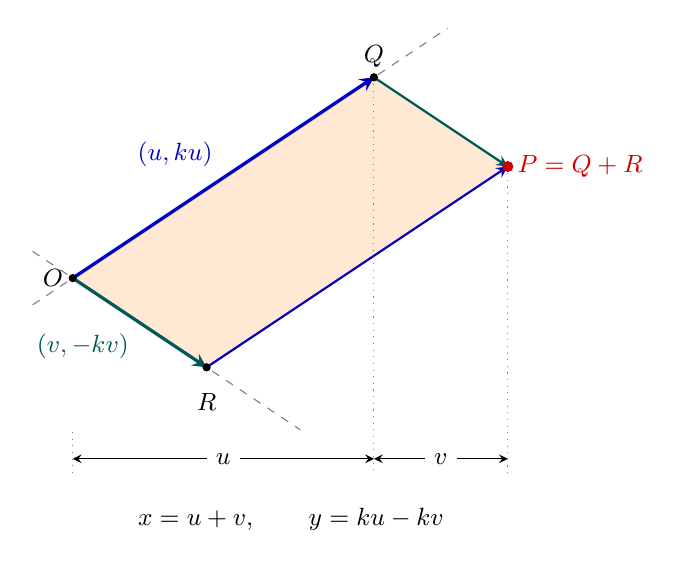
\begin{tikzpicture}[x=1.7cm,y=1.7cm,>=stealth,font=\small]
\coordinate (O) at (0,0); \coordinate (Q) at (2.25,1.5);
\coordinate (R) at (1,-2/3); \coordinate (P) at (3.25,5/6);
\fill[orange!17] (O)--(Q)--(P)--(R)--cycle;
\draw[gray,dashed] (-.3,-.2)--(2.8,28/15);
\draw[gray,dashed] (-.3,.2)--(1.7,-17/15);
\draw[->,blue!75!black,very thick] (O)--(Q) node[midway,above left] {$(u,ku)$};
\draw[->,teal!70!black,very thick] (O)--(R) node[midway,below left] {$(v,-kv)$};
\draw[->,teal!70!black,thick] (Q)--(P);
\draw[->,blue!75!black,thick] (R)--(P);
\draw[gray,dotted] (0,-1.15)--(0,-1.45) (Q)--(2.25,-1.45) (P)--(3.25,-1.45);
\draw[<->] (0,-1.35)--(2.25,-1.35) node[midway,fill=white] {$u$};
\draw[<->] (2.25,-1.35)--(3.25,-1.35) node[midway,fill=white] {$v$};
\node at (1.63,-1.8) {$x=u+v,\qquad y=ku-kv$};
\fill (O) circle(1.5pt) node[left] {$O$};
\fill (Q) circle(1.5pt) node[above] {$Q$};
\fill (R) circle(1.5pt) node[below=6pt] {$R$};
\fill[red!80!black] (P) circle(2pt) node[right] {$P=Q+R$};
\end{tikzpicture}

\end{center}

记 $k=b/a$，分别把 $OQ$、$OR$ 端点写为
\[
Q=(u,ku),\qquad R=(v,-kv).
\]
因为 $OQPR$ 是平行四边形，$P=Q+R$，所以
\[
x=u+v,\qquad \frac yk=u-v.
\]
\textbf{第1步：}双曲线方程改写为 $x^2-y^2/k^2=a^2$，于是
\[
\boxed{4uv=(u+v)^2-(u-v)^2=a^2}.
\]
\textbf{第2步（纯底高，不用行列式）：}考虑\textbf{竖直剪切}
$(X,Y)\mapsto(X,Y-kX)$，它使每条竖直截线只上下移动，截线长度不变，
故面积保持不变。剪切后三个顶点成为
\[
O'=(0,0),\qquad Q'=(u,0),\qquad R'=(v,-2kv).
\]
因平行四边形的第四点 $P'=Q'+R'$，
其底边 $O'Q'$ 是\textbf{水平}的，底长 $|u|$，高为 $2k|v|$，
直接用初中\emph{底乘高}：
\[
\boxed{S=|u|\times 2k|v|=2k|uv|}.
\]
这里没有求两条斜线的交点、点到斜线距离或行列式。
\textbf{第3步：}代入 $uv=a^2/4$：
\[
S=2k\cdot\frac{a^2}{4}=\boxed{\frac{ab}{2}}.
\]
\textbf{最小数值演示：}设 $a=3,b=2$，则 $k=2/3$、$uv=9/4$，
面积立即是 $2\cdot(2/3)\cdot(9/4)=3$，无论 $u,v$ 如何变化。
\textbf{为什么门槛低：}核心只有 $\boxed{(u+v)^2-(u-v)^2=4uv}$。

\textbf{不使用剪切的备用底高法：}
$|OQ|=|u|\sqrt{1+k^2}$；
把 $R$ 到 $OQ$ 的垂高表示为
$h=2k|v|/\sqrt{1+k^2}$（在 $R$ 所在横坐标处，
两条斜线 $y=\pm kX$ 的竖直间距为 $2k|v|$，
再乘以斜线与水平方向夹角的余弦）。
所以 $S=|OQ|\cdot h=2k|uv|$。
此法只需\emph{勾股定理与三角形相似／锐角三角函数}，不用行列式。
\end{proofbox}

\clearpage
\begin{proofbox}
\textbf{方法三：常规解析几何【直线交点坐标＋面积行列式】。}

图中 $k=b/a$，$(X,Y)$ 表示直线上的动点，$P=(x,y)$ 为给定点。

\begin{center}
% k=2/3 and P=(13/4,5/6); the labels give the general equations.
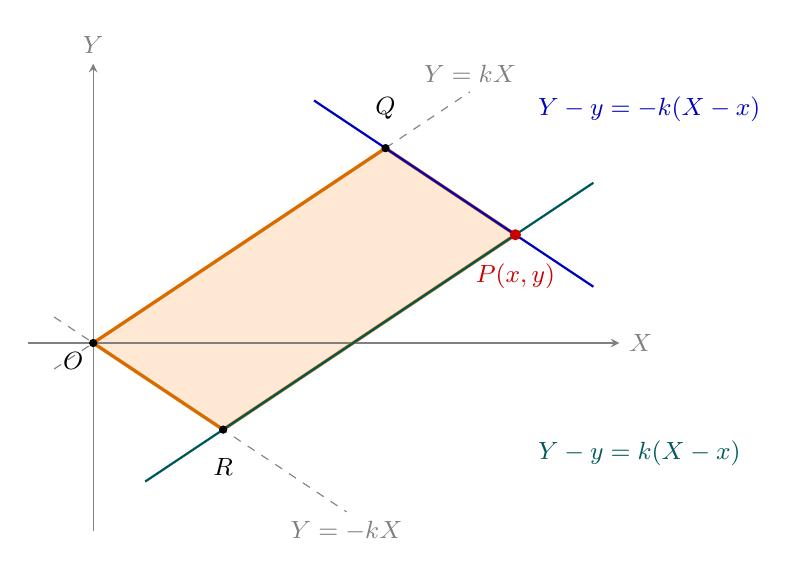
\begin{tikzpicture}[x=1.65cm,y=1.65cm,>=stealth,font=\small]
\coordinate (O) at (0,0); \coordinate (Q) at (2.25,1.5);
\coordinate (R) at (1,-2/3); \coordinate (P) at (3.25,5/6);
\fill[orange!17] (O)--(Q)--(P)--(R)--cycle;
\draw[->,gray] (-.5,0)--(4.05,0) node[right] {$X$};
\draw[->,gray] (0,-1.45)--(0,2.15) node[above] {$Y$};
\draw[gray,dashed] (-.3,-.2)--(2.9,29/15) node[above] {$Y=kX$};
\draw[gray,dashed] (-.3,.2)--(1.95,-1.3) node[below] {$Y=-kX$};
\draw[orange!85!black,very thick] (O)--(Q)--(P)--(R)--cycle;
\draw[blue!75!black,thick] (1.7,28/15)--(3.85,13/30);
\draw[teal!70!black,thick] (.4,-16/15)--(3.85,37/30);
\node[anchor=west,blue!75!black] at (3.35,1.8) {$Y-y=-k(X-x)$};
\node[anchor=west,teal!70!black] at (3.35,-.85) {$Y-y=k(X-x)$};
\fill (O) circle(1.5pt) node[below left] {$O$};
\fill (Q) circle(1.5pt) node[above=7pt] {$Q$};
\fill (R) circle(1.5pt) node[below=7pt] {$R$};
\fill[red!80!black] (P) circle(2pt) node[below=7pt] {$P(x,y)$};
\end{tikzpicture}

\end{center}

\textbf{第1步：}联立渐近线与过 $P$ 的平行线。设
$Q\in\ell_+$、$R\in\ell_-$，且 $\overrightarrow{PQ}\parallel\ell_-$、
$\overrightarrow{PR}\parallel\ell_+$，解得
\[
\boxed{Q\left(\frac{x}{2}+\frac{ay}{2b},\ \frac{bx}{2a}+\frac y2\right)},
\quad
\boxed{R\left(\frac{x}{2}-\frac{ay}{2b},\ -\frac{bx}{2a}+\frac y2\right)}.
\]
验证 $Q+R=(x,y)=P$，说明四边形确为平行四边形。

\textbf{第2步：}以 $OQ$、$OR$ 为邻边取行列式：
\[
\begin{aligned}
S&=|x_Qy_R-y_Qx_R|\\
 &=\left|\frac{a}{2b}y^2-\frac{b}{2a}x^2\right|\\
 &=\frac{ab}{2}\left|\frac{x^2}{a^2}-\frac{y^2}{b^2}\right|
 =\boxed{\frac{ab}{2}}.
\end{aligned}
\]
\textbf{常规法优势：}给出 $Q,R$ 的\textbf{准确位置}，
可继续求边长、周长、顶点坐标等，不只解决面积问题。
\end{proofbox}

\clearpage
\begin{proofbox}
\textbf{方法四：向量／仿射坐标法【补充：识别一般二次曲线的不变量】。}

\begin{center}
% Coefficient plane and physical plane; a=3,b=2,lambda=3/4,mu=1/3.
\begin{tikzpicture}[>=stealth,font=\small]
\begin{scope}[x=2.5cm,y=2.5cm]
\fill[orange!17] (0,0) rectangle (.75,1/3);
\draw[->,gray] (-.15,0)--(1,0) node[right] {$\lambda$};
\draw[->,gray] (0,-.15)--(0,.65) node[above] {$\mu$};
\draw[orange!85!black,thick] (0,0) rectangle (.75,1/3);
\fill[red!80!black] (.75,1/3) circle(2pt) node[above right] {$(\lambda,\mu)$};
\node at (.4,-.45) {系数平面：面积 $|\lambda\mu|$};
\end{scope}
\draw[->,thick] (3.5,.5)--(4.5,.5) node[midway,above] {$T$};
\begin{scope}[shift={(5.3,.2)},x=1.1cm,y=1.1cm]
\fill[orange!17] (0,0)--(2.25,1.5)--(3.25,5/6)--(1,-2/3)--cycle;
\draw[->,blue!75!black,thick] (0,0)--(3,2) node[above] {$\mathbf e_+$};
\draw[->,teal!70!black,thick] (0,0)--(3,-2) node[below] {$\mathbf e_-$};
\draw[orange!85!black,very thick] (0,0)--(2.25,1.5)--(3.25,5/6)--(1,-2/3)--cycle;
\node[above left] at (2.25,1.5) {$Q$};
\node[below] at (1,-2/3) {$R$};
\node[right] at (3.25,5/6) {$P$};
\node[left] at (0,0) {$O$};
\node at (1.7,-2.8) {原平面：面积 $2ab|\lambda\mu|$};
\end{scope}
\end{tikzpicture}

\end{center}

图中 $T(\lambda,\mu)=\lambda\mathbf e_++\mu\mathbf e_-$ 把矩形映成目标平行四边形。令
\[
\mathbf e_+=(a,b),\quad\mathbf e_-=(a,-b),\quad
P=\lambda\mathbf e_++\mu\mathbf e_-.
\]
于是
\[
\lambda=\frac12\left(\frac xa+\frac yb\right),\qquad
\mu=\frac12\left(\frac xa-\frac yb\right),
\quad 4\lambda\mu=\frac{x^2}{a^2}-\frac{y^2}{b^2}=1.
\]
两条邻边为 $\lambda\mathbf e_+$、$\mu\mathbf e_-$，所以
\[
S=|\lambda\mu|\,|\det(\mathbf e_+,\mathbf e_-)|
=\frac14\cdot 2ab=\boxed{\frac{ab}{2}}.
\]
\textbf{通式推广：}若 $x^2/a^2-y^2/b^2=t$，
则 $4\lambda\mu=t$，面积自然变为
\[
\boxed{S=\frac{ab}{2}|t|}.
\]
\textbf{迁移价值：}定值的本质是双曲线在渐近线方向上的两个\textbf{斜坐标乘积}恒定，
而面积正比于该乘积。
\end{proofbox}


\clearpage
\begin{proofbox}
\textbf{衍生性质一：邻边乘积定值、周长最小与菱形条件。}

令 $k=b/a$，由方法二知 $uv=a^2/4>0$，故 $u,v$ 同号。
两邻边长度为
\[
A=\sqrt{u^2+k^2u^2}=|u|\sqrt{1+k^2},\quad
B=|v|\sqrt{1+k^2}.
\]
利用 $c^2=a^2+b^2$：
\[
\boxed{AB=(1+k^2)|uv|=\frac{a^2+b^2}{4}=\frac{c^2}{4}}.
\]
于是
\[
\boxed{L=2(A+B)\ge4\sqrt{AB}=2c}.
\]
等号成立当且仅当 $A=B$，即 $|u|=|v|$。
因 $uv>0$，二者同号，所以 $u=v$，从而
$y=k(u-v)=0$；代入双曲线得 $x=\pm a$。
反之 $P=(\pm a,0)$ 时 $Q,R$ 关于 $x$ 轴对称且 $A=B$。
故\textbf{周长取最小值 $2c$}\emph{当且仅当} $P$ 为左右顶点，
此时恰为菱形；若还要求正方形，需额外 $a=b$。

\medskip
\textbf{衍生性质二：固定 $c$ 时的面积上界（含等号条件）。}
由 $(a-b)^2\ge0$，
\[
2ab\le a^2+b^2=c^2\quad\Longrightarrow\quad
\boxed{0<S=\frac{ab}{2}\le\frac{c^2}{4}}.
\]
等号当且仅当 $a=b=c/\sqrt2$；下界 $0$ 仅可逼近、不能达到（$a,b>0$）。
请区分：\emph{固定一条双曲线时面积恒定}，
与\emph{固定 $c$、改变 $a,b$ 时寻找面积最大值}是两个不同问题。
\end{proofbox}

\clearpage
\begin{proofbox}
\textbf{可迁移的统一定理：一次式乘积的等值曲线。}

设两个独立的一次式
\[
L_1(X,Y)=p_1X+q_1Y+r_1,\qquad
L_2(X,Y)=p_2X+q_2Y+r_2,
\]
且 $D=p_1q_2-q_1p_2\ne0$。直线 $L_1=0,L_2=0$
交于 $O$；过点 $P$ 分别作直线 $L_1=L_1(P)$、$L_2=L_2(P)$，
与原两条直线围成平行四边形（或退化情形）。则
\[
\boxed{S(P)=\frac{|L_1(P)L_2(P)|}{|D|}}.
\]
\textbf{证明（坐标映射）：}取新坐标 $U=L_1(X,Y)$、$V=L_2(X,Y)$。
原两条直线变为 $U=0$、$V=0$；过 $P$ 的平行线
变为 $U=L_1(P)$、$V=L_2(P)$，围成\emph{面积
$|L_1(P)L_2(P)|$ 的矩形}。线性坐标变换面积缩放倍数为 $|D|$，
故原面积除以 $|D|$ 得证。

\textbf{立即应用：}取
\[
L_1=\frac xa+\frac yb,\qquad
L_2=\frac xa-\frac yb,\qquad
D=-\frac{2}{ab}.
\]
则 $L_1L_2=x^2/a^2-y^2/b^2$；
沿 $L_1L_2=t$ 移动时面积恒为
\[
\boxed{S=\frac{|t|}{2/(ab)}=\frac{ab}{2}|t|}.
\]
\textbf{推广意义：}平移或旋转后的曲线，只要仍能写成
$L_1L_2=K$（且 $D\ne0$），便有面积定值 $|K|/|D|$。
\textbf{边界：}$D=0$ 时两条直线方向平行，不能照搬该公式；
$K=0$ 时图形退化为零面积。
\end{proofbox}
